\chapter{结果与讨论}
\label{chap:results}

\section{表格与结果呈现}

表~\ref{tab:main-results} 展示了三线表、表注和交叉引用方式。标题在表格上方，标签命令应紧跟表题命令。表内小字号、加粗表头和无编号表注是本示例的排版选择，学校规范未统一规定。

\begin{table}[htbp]
  \centering
  \small
  \caption{示例结果汇总}
  \label{tab:main-results}
    \begin{tabular}{lcc}
      \toprule
      \textbf{方法} & \textbf{指标一} & \textbf{指标二} \\
      \midrule
      基线方法 & 0.72 & 12.4 \\
      提出方法 & 0.85 & 9.1 \\
      \bottomrule
    \end{tabular}
  \thesistablenote{数据仅用于演示三线表结构，请替换为实际实验结果。表注可解释缩写、统计检验、单位或数据来源。}
\end{table}

表~\ref{tab:wide-table} 演示 \texttt{tabularx} 的宽表写法。长文字放入 \texttt{Y} 列，避免通过缩小字号或压缩列间距强行塞入内容。

\begin{table}[htbp]
  \centering
  \small
  \caption{示例宽表}
  \label{tab:wide-table}
  \begin{tabularx}{\textwidth}{lYY}
    \toprule
    \textbf{项目} & \textbf{说明} & \textbf{报告建议} \\
    \midrule
    数据集 & 说明数据来源、时间范围、样本量与筛选规则。 & 报告训练、验证和测试集的划分方式。 \\
    实验设置 & 说明硬件、软件版本、关键参数及随机种子。 & 保证他人能够复现主要结果。 \\
    评价指标 & 给出指标定义、单位、方向和统计方法。 & 同时报告均值、波动或置信区间。 \\
    \bottomrule
  \end{tabularx}
\end{table}

\section{子图与算法}

当多个面板共同回答一个问题时，使用图~\ref{fig:subfigures} 这样的子图。若各图相互独立，应拆成多张图，不要为节省页数强行拼接。

\begin{figure}[htbp]
  \centering
  \begin{subfigure}[b]{0.48\textwidth}
    \centering
    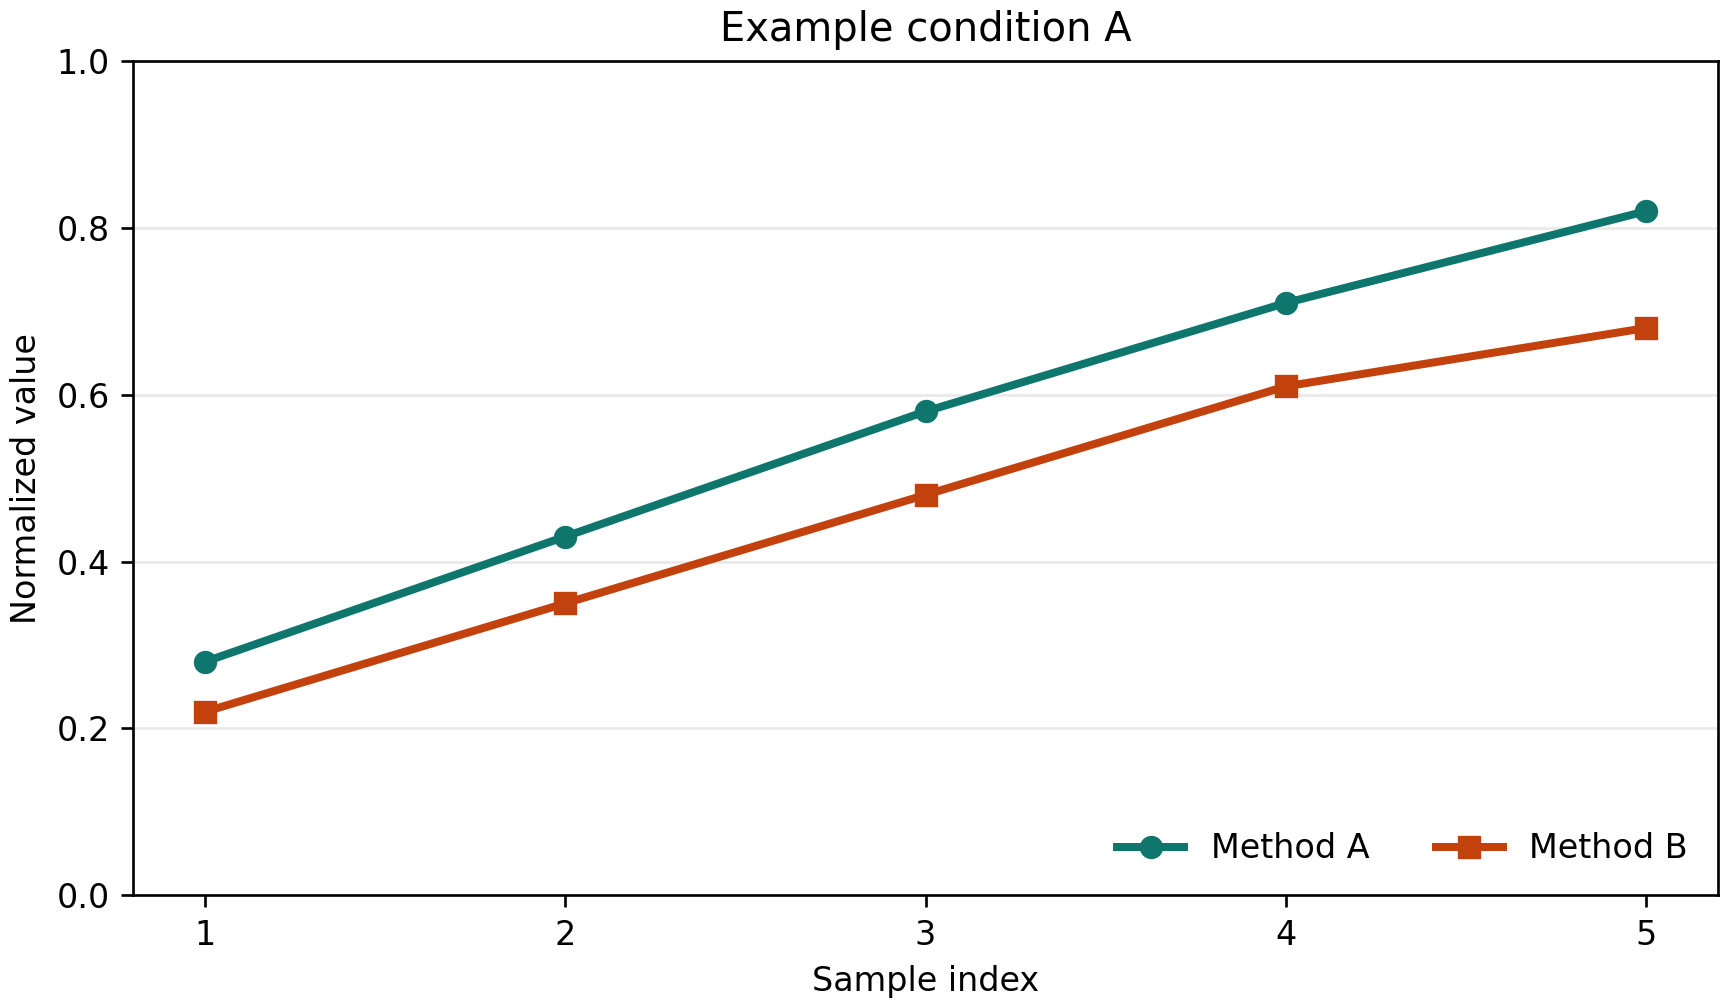
\includegraphics[width=\linewidth]{example-plot-a}
    \caption{}
    \label{fig:condition-a}
  \end{subfigure}
  \hfill
  \begin{subfigure}[b]{0.48\textwidth}
    \centering
    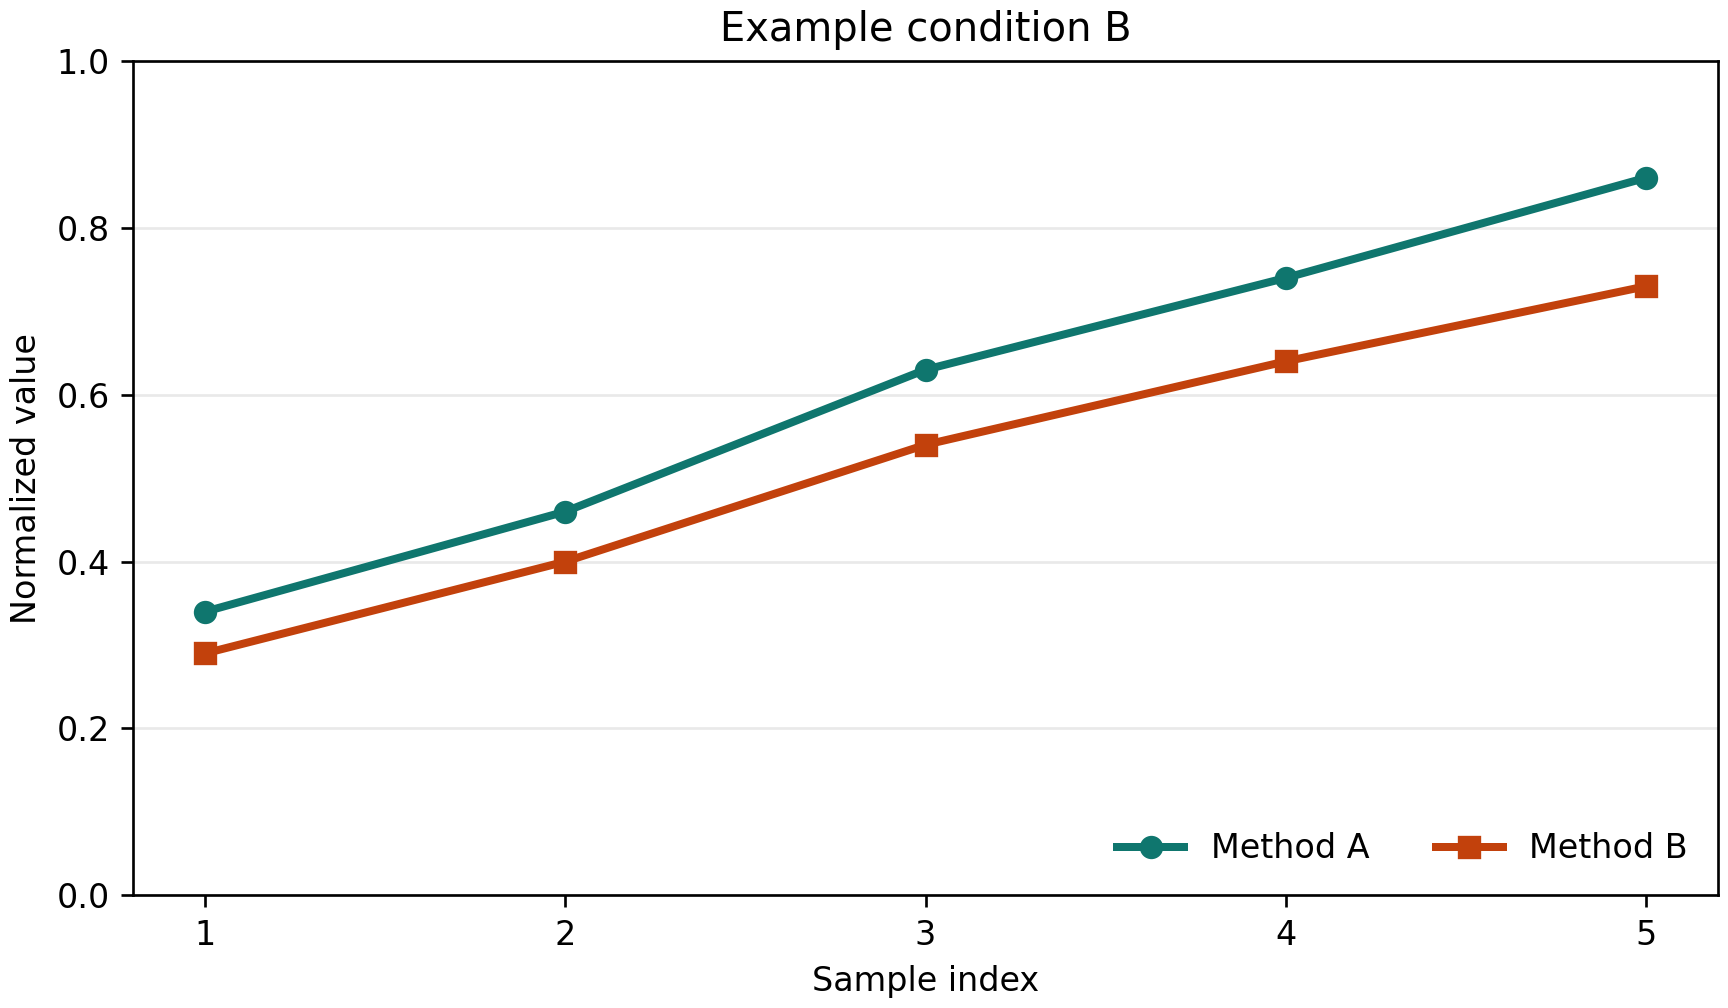
\includegraphics[width=\linewidth]{example-plot-b}
    \caption{}
    \label{fig:condition-b}
  \end{subfigure}
  % 组合图的插图清单名称写在总图题的方括号中。
  \caption[两种条件比较]{同一研究问题下的两种条件比较：（a）示例条件 A；（b）示例条件 B}
  \label{fig:subfigures}
\end{figure}

算法~\ref{alg:example} 演示伪代码环境。不要用截图展示算法；每一步应能与正文的输入、输出和符号对应。

\begin{algorithm}[htbp]
  \caption{示例处理流程}
  \label{alg:example}
  \begin{algorithmic}[1]
    \Require 输入数据集合 $\mathcal{D}$，阈值 $\tau$
    \Ensure 处理后的结果集合 $\mathcal{R}$
    \State 初始化 $\mathcal{R}\gets\varnothing$
    \For{每个样本 $d\in\mathcal{D}$}
      \State 计算评分 $s\gets f(d)$
      \If{$s\geq\tau$}
        \State 将 $d$ 加入 $\mathcal{R}$
      \EndIf
    \EndFor
    \State \Return $\mathcal{R}$
  \end{algorithmic}
\end{algorithm}
